\documentclass{article}
\usepackage{doc}

\begin{document}

% 标题
\title{io模块}
\maketitle

\begin{abstract}
    本文描述io模块的设计与实现
\end{abstract}

\tableofcontents
\vskip\baselineskip

io模块提供对文件、网络io的封装。系统原本打算直接使用boost::asio作为io框架，但是由于项目关闭了异常，导致asio无法正常编译，所以只能自己实现一个io框架。

\section{异步框架}

异步框架模仿asio的设计，其核心是一个task queue队列，每个task是一个异步操作。线程池中的线程会从队列中取出task执行，另一侧是reactor由系统epoll事件触发，将事件封装成task并加入队列。这是一个典型的生产者-消费者模型。

\begin{figure}[H]
    \centering
    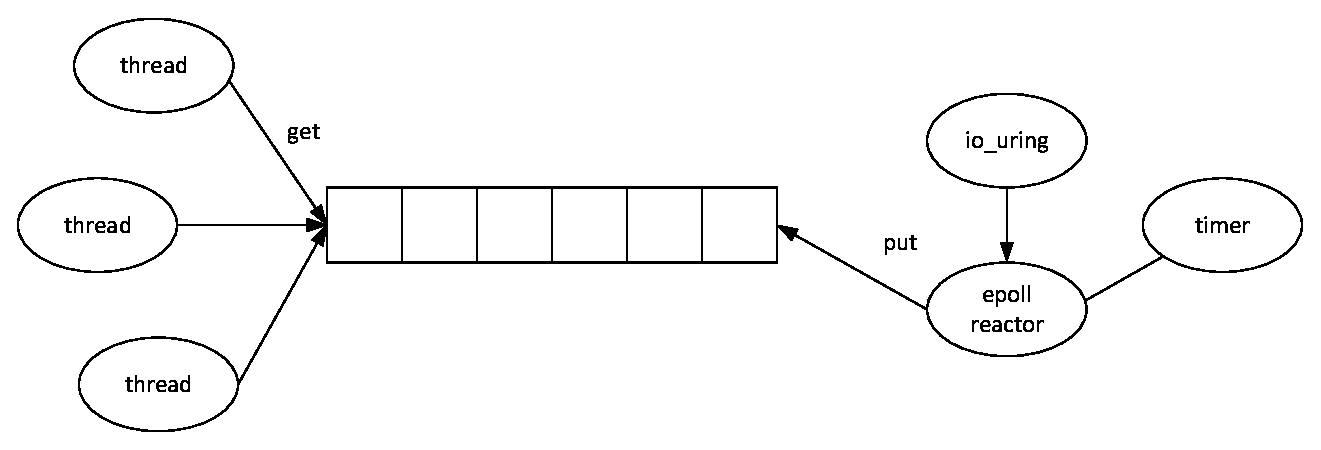
\includegraphics[width=\linewidth]{img/io/i-arch.eps}
    \caption{异步框架}\label{fig:i-arch}
\end{figure}

这个异步框架的执行单位是异步task，线程是执行对象。线程的诞生，将cpu管理从进程中剥离出来，多个线程可以并发执行。但是这并非没有的代价，线程维护开销与切换开销不小。这个异步框架，以线程表达cpu算力，由异步task表示计算任务，要求异步任务不得阻塞线程执行，这样就能避免cpu的算力被浪费。

异步task用函数来表示，函数内部有可能调用阻塞io操作，c++20协程可以在函数中异步等待io操作完成，而不阻塞线程。所以，虽然\figurename\ref{fig:i-arch}构架中是一个异步任务为调度单位，但用户最好使用协程，以防调用阻塞io操作。

对数据库而言，每个会话对应一个协程，协程内部执行SQL语句。在\figurename\ref{fig:i-coro}中，底层是异步框架。当客户连接进来后，指派一个协程去运行session会话，又该会话代理SQL语句的执行。

\begin{figure}[H]
    \centering
    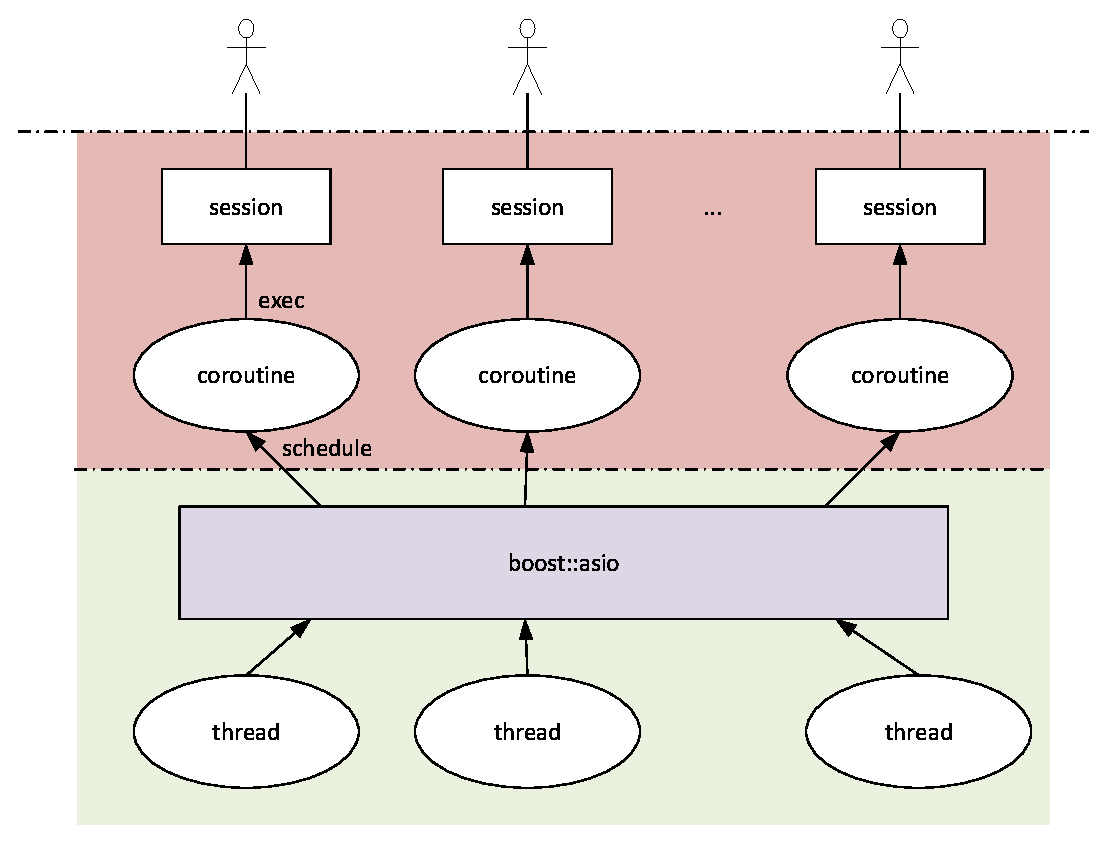
\includegraphics[width=\linewidth]{img/io/i-coro.eps}
    \caption{waterfall协程架构}\label{fig:i-coro}
\end{figure}

\section{executor}

按照\figurename\ref{fig:i-arch}模型，一个异步任务执行的上下文场景是多变的，目前至少有两种场景：一种是全局调度器，一种是strand。strand保证异步任务串行执行，无需使用线程mutex变量，减轻了程序员负担。

unifex\cite{GitHubfa18:inline}假设在编译时刻知道executor的类型，它的执行器都是在编译时刻静态绑定的。waterfall假定执行器是动态的，例如，当一个异步任务先假定在gpu上执行，后来运行时刻场景变换，需要切换到cpu上执行，这在编译时刻是不能确定的。并且，从实现层面上看，unifex的静态绑定开销其实不小，构造的静态vtable其实仍然需要一个函数指针转发。

\begin{lstlisting}[style=c++]
// 运行时执行器接口
struct runtime_executor
{
    virtual ~runtime_executor() = default;
    virtual void execute(async_task &task) = 0;
    virtual void execute(task_queue &queue) = 0;
};
\end{lstlisting}

执行器接口很简单，只有两个方法，分别是执行一个异步任务和执行一个任务队列。这里不装了，asio中operation是一个非常重要的抽象，它将异步操作封装成一个队列，开销比较少。这种封装是否足够通用？有待观察，例如gpu场景下，gpu是否支持后继指针？

在\figurename\ref{fig:i-arch}模型中，一个线程可以进入多种执行场景，最底层是全局调度器，栈上的执行器以链表形式组织起来，当前执行器由一个thread\_local变量指定，如\figurename\ref{fig:i-executor}所示。

\begin{figure}[H]
    \centering
    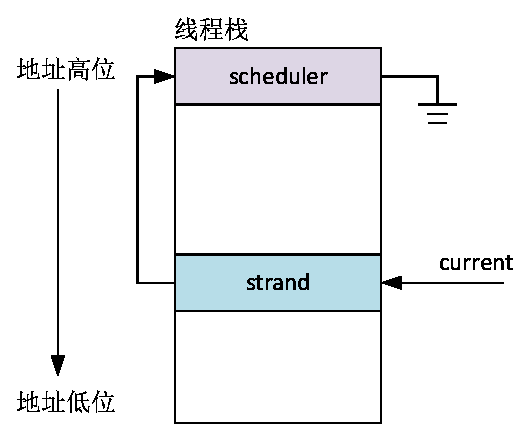
\includegraphics[width=0.5\linewidth]{img/io/i-executor.eps}
    \caption{线程栈上的执行器链表}\label{fig:i-executor}
\end{figure}

\section{协程}

c++20协程定义为一种特殊的函数，当函数内碰到co\_return、co\_yield、co\_await三个关键字，该函数为一个协程。协程与普通函数有如下区别：
\begin{itemize}
    \item 协程的执行模型是堆而非栈。协程要求重入，考虑函数重入，需要将栈帧来回拷贝，或者保留整个栈帧。如果保留整个栈桢，还需要切换寄存器组。合计下来，不如直接将协程处理为堆上的对象。
    \item 协程的执行模型为堆，编译器要在编译期计算协程帧的大小，这个其实挺不容易，需要枚举所有执行流程，计算出最大内存分配。好消息是，局部变量的声明总是有数的。
    \item 除了局部变量，协程帧还需保存重入位置，调用参数等。
\end{itemize}

调用一个协程形如调用一个普通函数，但编译器要求直接返回对象内部必须声明一个promise\_type类，这个类是协程用户定制的协程控制块，后续协程的动作会根据这个类的方法来进行。

\subsection{awaiter}

如果按照状态划分，协程可以分为挂起、执行两种状态。协程需要自愿挂起，无法抢断，因为协程是在用户态实现，缺乏必要的机制。协程执行到挂起点，会在协程帧上执行挂起点的awaiter，编译器要求awaiter提供三个方法：
\begin{itemize}
    \item await\_ready。判断awaiter是否ready，ready表示可以直接执行awaiter的await\_resume方法，否则需要挂起协程。
    \item await\_suspend。挂起协程，将协程帧加入到等待队列中。
    \item await\_resume。恢复协程执行，返回awaiter的结果。
\end{itemize}

三个方法的调用关系如\figurename\ref{fig:i-suspend}所示。根据await\_ready的返回值，判定是否可以挂起或者resume，await\_resume函数会执行一系列动作恢复协程的执行。

\begin{figure}[H]
    \centering
    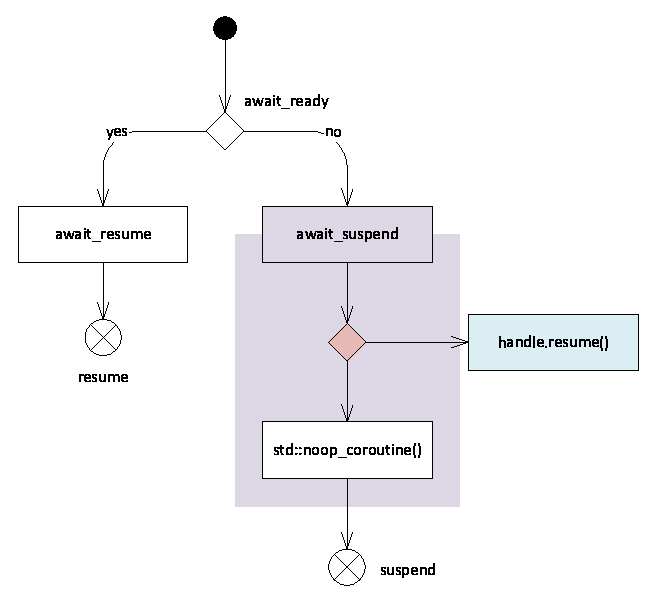
\includegraphics[width=0.8\linewidth]{img/io/i-suspend.eps}
    \caption{复杂的await\_suspend}\label{fig:i-suspend}
\end{figure}

await\_resume还需要特别注意的是，这两个函数是有返回值的。例如，当一个协程执行auto ret = await long\_op指令，协程根据long\_op返回值拿到一个awaiter，然后执行await\_resume方法，await\_resume的返回值被放在了ret变量。除了co\_await外，还有co\_yield可能拿到awaiter的返回值。

await\_suspend比较麻烦，这个函数带了一个coroutine\_handle参数，这是该协程的句柄，根据这个局部可以访问协程的promise，从而可以做复杂的逻辑判断。并且，await\_suspend有多种返回值，如果它返回一个协程句柄handle，会调用该句柄handle.resume()恢复协程执行。如果handle是该协程，就会恢复协程执行。如果是std::noop\_coroutine()返回的句柄，则挂起该协程。

最后，关于awaiter需要注意的是，awaiter放在协程堆上，执行的主体是该协程。

\subsection{awaitable}

当协程执行如下两条语句时，先执行expr，返回一个对象，称为awaitable。协程需要根据awaitable生成一个awaiter对象，然后再执行awaiter。

\begin{lstlisting}[style=c++,frame=none,numbers=none,backgroundcolor=\color{gray!20}]
co_yield expr;
co_await expr;
\end{lstlisting}

从awaitable转awaiter的动作是编译器执行，编译器根据两种情况转换：
\begin{itemize}
    \item awaitable对象重载了co\_await运算符，返回一个awaiter对象。
    \item 或者promise\_type里实现了await\_transform方法，将awaitable变换为一个awaiter。
\end{itemize}

为增加库的弹性，定制了一个

\subsection{挂起点}

协程的挂起点有4个：

\begin{itemize}
    \item initial\_suspend。调用一个协程，编译器插入一段初始化协程的代码，协程帧构造完毕后会会调用initial\_suspend，为caller提供一个选择如何调度协程的机会。
    \item final\_suspend。协程执行完毕，会调用final\_suspend，以便通知caller。
    \item co\_await。这条指令的含义也很丰富：
\begin{lstlisting}[style=c++,frame=none,numbers=none,backgroundcolor=\color{gray!20}]
co_await op;
\end{lstlisting}
先执行op，op返回一个对象，称为awaitable。如果awaitable是一个awaiter，就直接执行awaiter。或者通过co\_await重载，或者通过await\_transform将awaitable变换为一个awaiter。awaitable之所以称为awaitable，就是因为可以得到awaiter。

op如果是一个异步操作，在当下会返回一个future这样的awaitable对象，最终转换为awaiter。如果op是一个同步操作，会等到op处理完毕后才返回awaitable。——协程需要用户编程，才是异步的。
    \item co\_yield。这条指令的目的是与caller交互，协程主动放弃执行，复杂的例子是父协程co\_await一个子协程，子协程co\_yield放弃执行，两个协程之间的协同如同化学反映，各种情况会爆炸。
\end{itemize}

\subsection{协程调度模式}

在\figurename\ref{fig:i-arch}框架下，协程有两种调度模式：本地调度和异步调度。本地调度是在该线程上继续执行协程，异步调度将协程作为一个task丢到任务队列中，由其它线程执行。

基于效率的考虑，本地调度是默认模式，异步调度需要显式指定，但有可能会产生starvation的情况。

\subsection{设计思路}

c++20协程标准非常开放，对协程库的设计不是一个好消息。waterfall的协程库要选定一种用户协程使用范式，然后根据这个范式来设计协程库。不太可能支持所有协程范式，这样对协程库的设计会很复杂。

协程库的使用范式主要参考golang、unifex两个协程库的设计。

\subsubsection{resume}

为了与调度器匹配，协程的promise从async\_task派生，因此协程天然就是一个异步任务，一个可重入的异步任务。

协程的恢复分为两种情况，一种是inline，一种是offline，前者调用std::coroutine的resume方法，后者需要先将协程加入到任务队列中，然后由executor来恢复协程执行。需要说明，std::coroutine\_handle的resume方法根据协程挂起的位置重入执行，这个函数用于实现inline恢复，它是编译器生成，无法修改。

promise保存了协程是否offline状态，缺省构造是inline，可以在initial\_suspend挂起后，指定为offline。promise提供统一的resume方法，这个方法根据协程是否offline，选择调用inline\_resume或者offline\_resume。

\subsubsection{continuation}

当协程结束，有时会调用下一个协程，例如caller协程等待callee协程执行完毕，或者在链式处理中，下一个处理过程的协程要接过上一个协程的结果继续执行。

continuation指向下一个协程，问题是它是句柄好？还是promise指针好？选择句柄，有可能挂接其它类型协程。看考虑到promise必须提供inline/offline统一的调度方法，还是选择promise指针。

\subsubsection{await\_transform}

协程库提供了协程promise和coroutine\_type两个类模板，分别对应协程的承诺和协程的类型，这种封装使得协程的创建更简洁。但是这限制了协程库的弹性，尤其是当用户需要在协程中使用一些特殊的awaitable对象时。waterfall从unifex偷师了await\_transform的cpo，允许用户通过await\_tranform定制awaitable对象的转换。

\subsubsection{return\_value/return\_void}

处理协程的返回值。

\subsubsection{initial\_suspend}

协程创建会调用initial\_suspend，为caller提供一个选择如何调度协程的机会。协程缺省是inline的，可以在创建后设置为offline，也可以绑定协程的执行器，指定协程完成后的contination协程等。

系统提供两种awaiter：initial\_suspend\_unready和initial\_suspend\_ready，在async\_promise模板中，缺省是initial\_suspend\_unready。

\subsubsection{final\_suspend}

协程执行完毕，会调用final\_suspend函数，返回一个awaiter。多数情况下，为了获取协程的返回值，返回的awaiter是final\_suspend\_unready。少数情况下，caller启动一个协程，然后detach该协程，由协程自己完成后销毁。

\subsubsection{yield\_value}

协程在执行co\_yield expr语句时，expr返回值是一个awaitable对象，被转换成awaiter，然后根据awaiter动作。yield\_value输入是






% 参考文献
\printbibliography

% 附录
\appendix

\end{document}